\begin{itemize}
	
\item{} Locate observation in archive - \url{http://kat-archive.kat.ac.za:8080/archive\_search/}
\item{} Inspect obs report
\item{} Rate the observation according to QA standards -\url{ http://ops.kat.ac.za/qa/}
\item{} Log or open a JIRA on problems picked up from the report for follow up
\item{} Report to the AoD.
\end{itemize}
\section{ Files status via SDP MC dashboard} 
If an operator fails to find data files in the archive, before raising a report:
\begin{itemize}
\item[\textbf{Step 1}] On your preferred browser, go to \url{http://mc1.sdp.mkat.karoo.kat.ac.za:5004/}\\
This will take you to the menu as shown in \textbf{Figure}~\ref{fig:image96}
\begin{figure}[!thb]
	\centering
	%\includegraphicsdpi{100}{}{bur1.png}     
	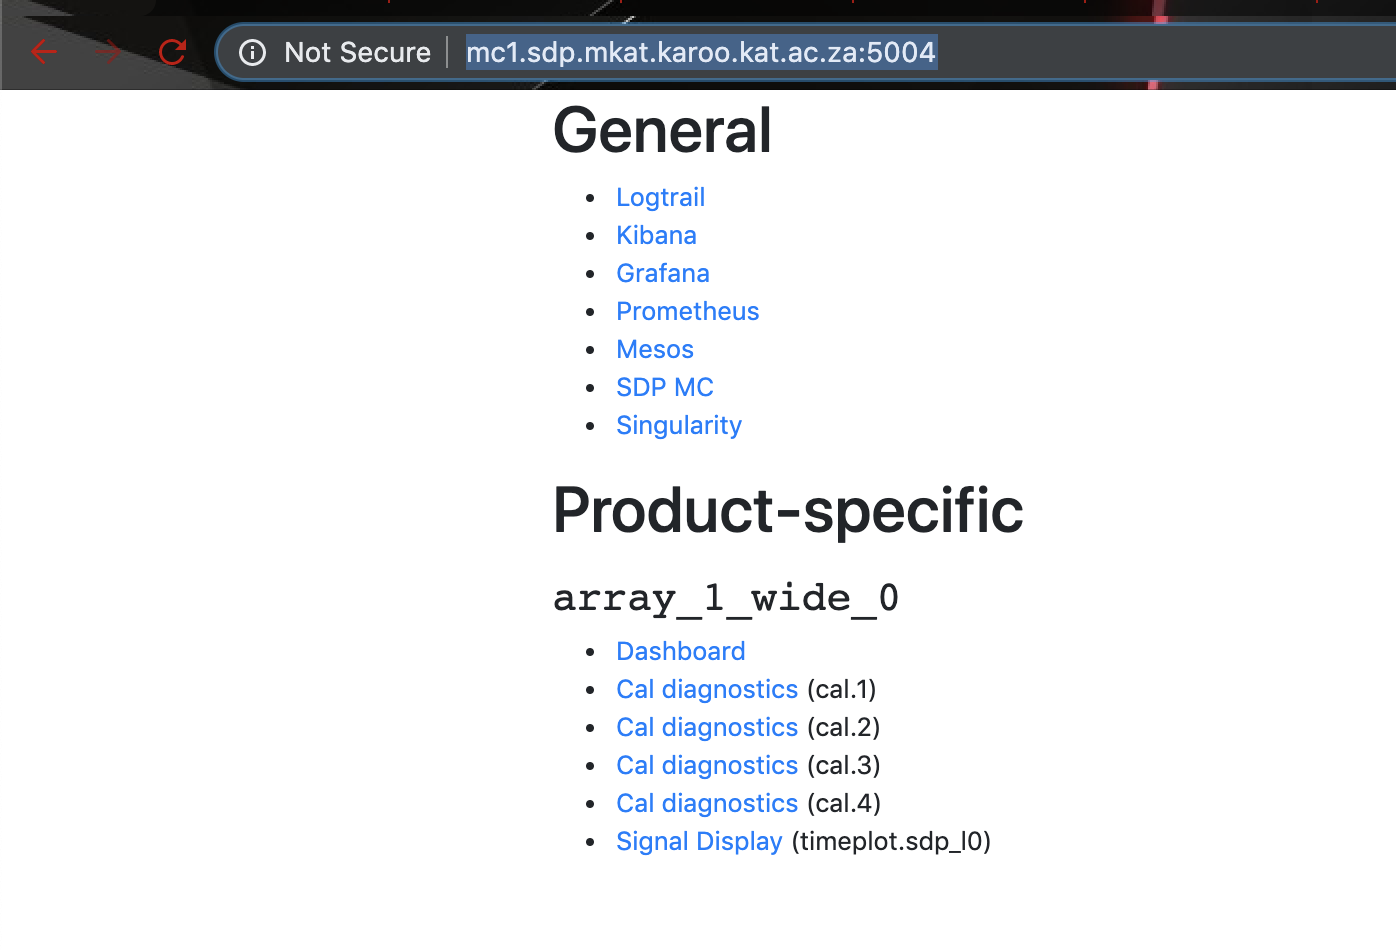
\includegraphics[scale=0.33]{Chapters/images/image96.png}
	
	%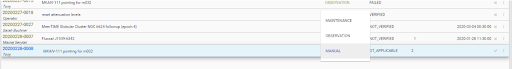
\includegraphics[resolution=100]{bur1.png}
	\caption{SDP main menu}
	\label{fig:image96}
\end{figure}


\item[\textbf{Step 2}] Click on DASHBOARD,  this will take you to sdp dashboard as shown in \textbf{Figure}~\ref{fig:image16}:


\begin{figure}[!thb]
	\centering
	%\includegraphicsdpi{100}{}{bur1.png}     
	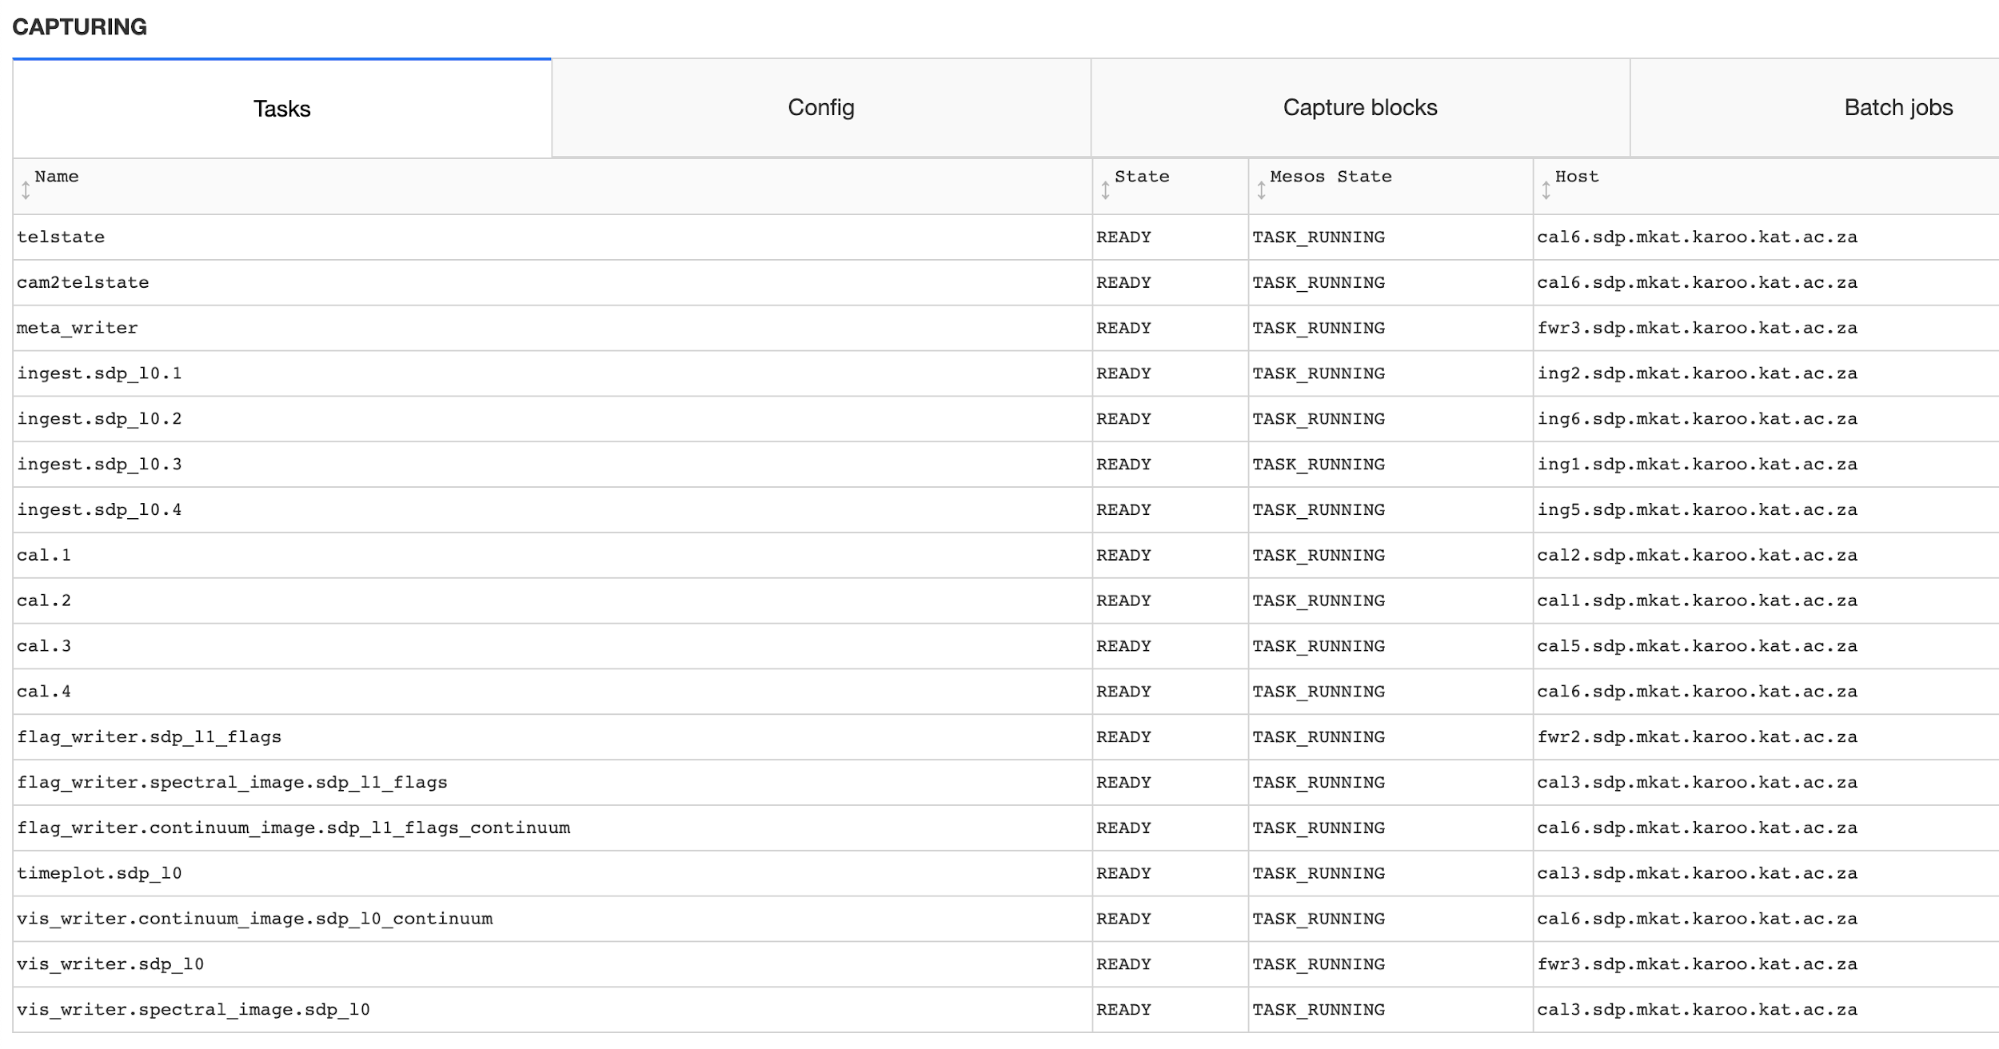
\includegraphics[scale=0.19]{Chapters/images/image16.png}
	
	%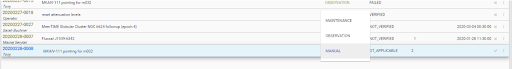
\includegraphics[resolution=100]{bur1.png}
	\caption{SDP Dashboard}
	\label{fig:image16}
\end{figure}

\begin{itemize}
	\item[$\circ$] Under MESOS STATE, you can see the status of the current observation
\end{itemize}


\item[\textbf{Step 3}] Go to CAPTURE BLOCKS, this will show \textbf{Figure}~\ref{fig:image5}.
\begin{itemize}
	\item[$\circ$] If there’s an Observation running(CAPTURING)


\begin{figure}[!thb]
	\centering
	%\includegraphicsdpi{100}{}{bur1.png}     
	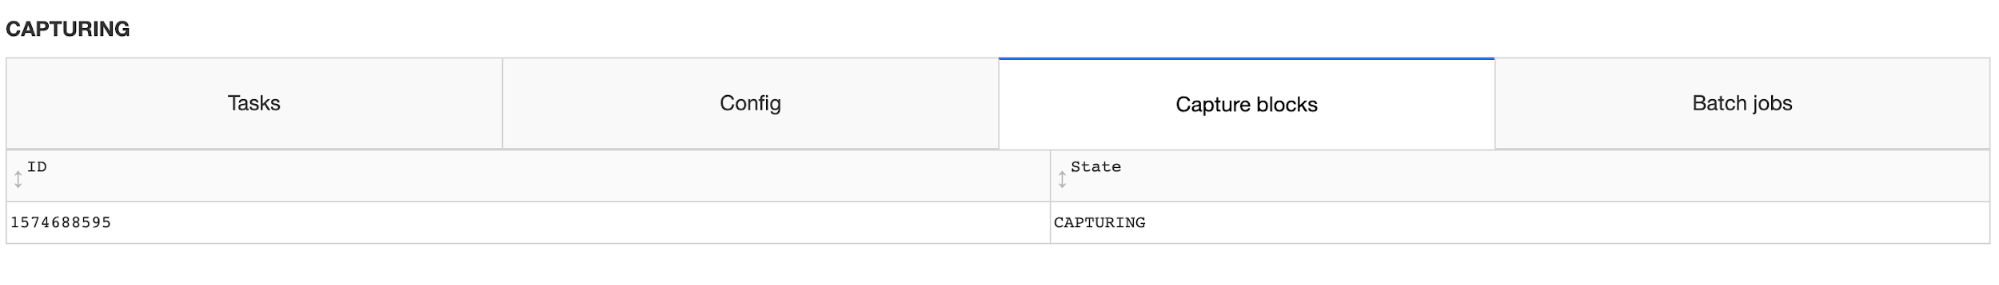
\includegraphics[scale=0.23]{Chapters/images/image5.png}
	
	%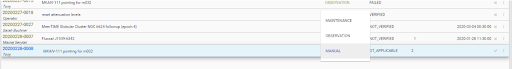
\includegraphics[resolution=100]{bur1.png}
	\caption{SDP Capturing}
	\label{fig:image5}
\end{figure}
\item[$\circ$] If an Observation just ended(POSTPROCESSING), see \textbf{Figure}~\ref{fig:image16} for status. 

\begin{figure}[!thb]
	\centering
	%\includegraphicsdpi{100}{}{bur1.png}     
	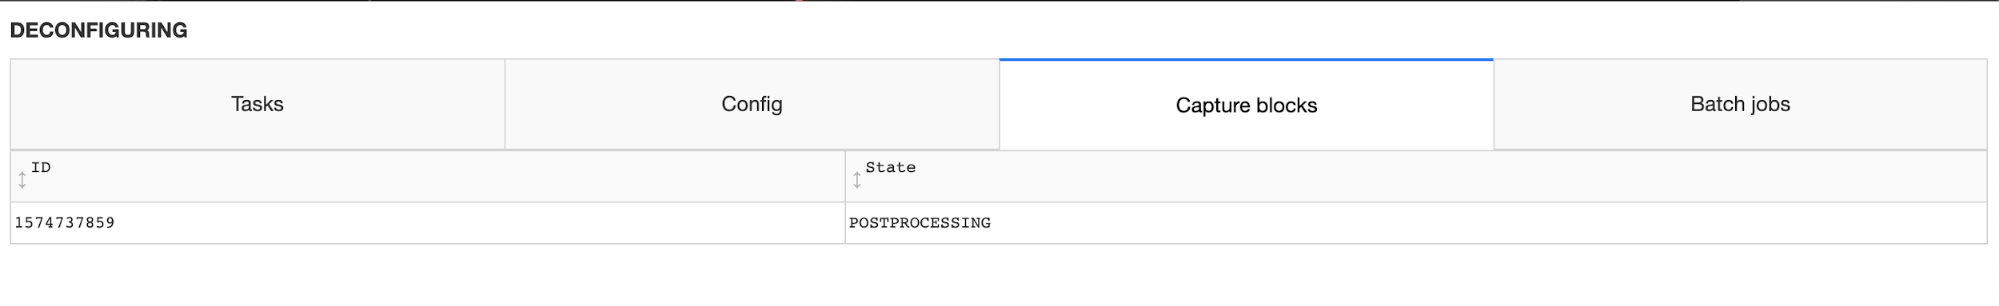
\includegraphics[scale=0.23]{Chapters/images/image92.png}
	
	%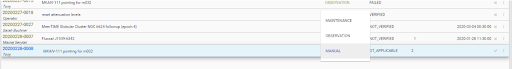
\includegraphics[resolution=100]{bur1.png}
	\caption{SDP Postprocessing}
	\label{fig:image92}
\end{figure}
\item[$\circ$] Under Batch Jobs you can view, under Runtime, the duration of the POSTPROCESSING process  as shown in \textbf{Figure}~\ref{fig:image13}.

\begin{figure}[!thb]
	\centering
	%\includegraphicsdpi{100}{}{bur1.png}     
	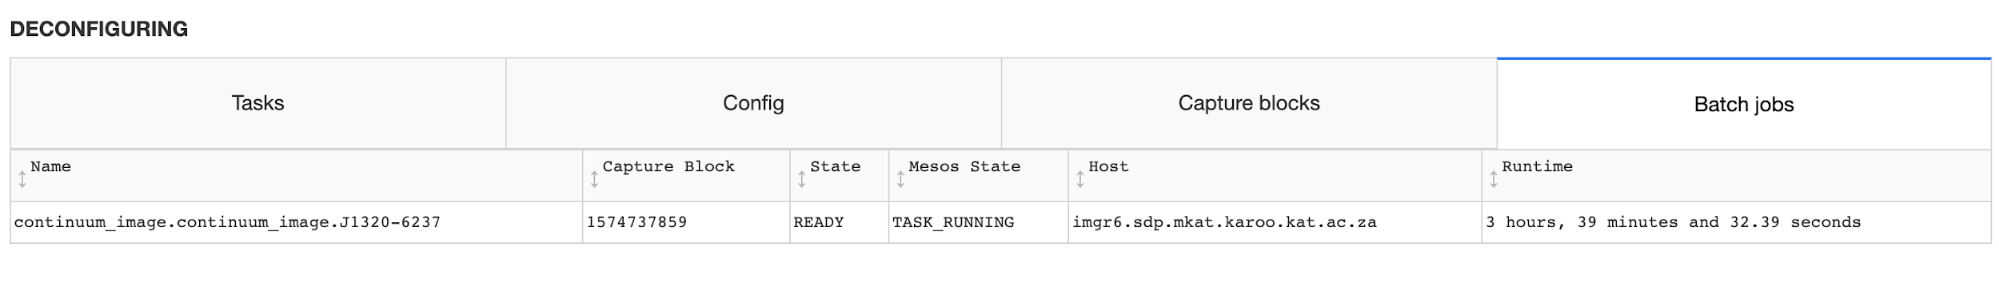
\includegraphics[scale=0.23]{Chapters/images/image13.png}
	
	%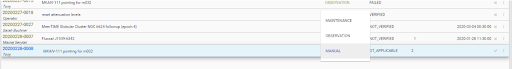
\includegraphics[resolution=100]{bur1.png}
	\caption{SDP batch jobs}
	\label{fig:image13}
\end{figure}
\item[$\circ$] Once it’s done with POSTPROCESSING go to the SARAO ARCHIVE to see if the observation is now in the archive(If not, report the issue in a JIRA.
\end{itemize}

\end{itemize}
Note: Duration for POSTPROCESSING depends on the duration of the observation. (Longer observations takes longer to go through the POSTPROCESSING process)






